\documentclass[]{article}
\usepackage{lmodern}
\usepackage{amssymb,amsmath}
\usepackage{ifxetex,ifluatex}
\usepackage{fixltx2e} % provides \textsubscript
\ifnum 0\ifxetex 1\fi\ifluatex 1\fi=0 % if pdftex
  \usepackage[T1]{fontenc}
  \usepackage[utf8]{inputenc}
\else % if luatex or xelatex
  \ifxetex
    \usepackage{mathspec}
  \else
    \usepackage{fontspec}
  \fi
  \defaultfontfeatures{Ligatures=TeX,Scale=MatchLowercase}
\fi
% use upquote if available, for straight quotes in verbatim environments
\IfFileExists{upquote.sty}{\usepackage{upquote}}{}
% use microtype if available
\IfFileExists{microtype.sty}{%
\usepackage{microtype}
\UseMicrotypeSet[protrusion]{basicmath} % disable protrusion for tt fonts
}{}
\usepackage[margin=1in]{geometry}
\usepackage{hyperref}
\hypersetup{unicode=true,
            pdftitle={DATA 605 - Assignment 15},
            pdfauthor={Joshua Sturm},
            pdfborder={0 0 0},
            breaklinks=true}
\urlstyle{same}  % don't use monospace font for urls
\usepackage{color}
\usepackage{fancyvrb}
\newcommand{\VerbBar}{|}
\newcommand{\VERB}{\Verb[commandchars=\\\{\}]}
\DefineVerbatimEnvironment{Highlighting}{Verbatim}{commandchars=\\\{\}}
% Add ',fontsize=\small' for more characters per line
\usepackage{framed}
\definecolor{shadecolor}{RGB}{248,248,248}
\newenvironment{Shaded}{\begin{snugshade}}{\end{snugshade}}
\newcommand{\AlertTok}[1]{\textcolor[rgb]{0.94,0.16,0.16}{#1}}
\newcommand{\AnnotationTok}[1]{\textcolor[rgb]{0.56,0.35,0.01}{\textbf{\textit{#1}}}}
\newcommand{\AttributeTok}[1]{\textcolor[rgb]{0.77,0.63,0.00}{#1}}
\newcommand{\BaseNTok}[1]{\textcolor[rgb]{0.00,0.00,0.81}{#1}}
\newcommand{\BuiltInTok}[1]{#1}
\newcommand{\CharTok}[1]{\textcolor[rgb]{0.31,0.60,0.02}{#1}}
\newcommand{\CommentTok}[1]{\textcolor[rgb]{0.56,0.35,0.01}{\textit{#1}}}
\newcommand{\CommentVarTok}[1]{\textcolor[rgb]{0.56,0.35,0.01}{\textbf{\textit{#1}}}}
\newcommand{\ConstantTok}[1]{\textcolor[rgb]{0.00,0.00,0.00}{#1}}
\newcommand{\ControlFlowTok}[1]{\textcolor[rgb]{0.13,0.29,0.53}{\textbf{#1}}}
\newcommand{\DataTypeTok}[1]{\textcolor[rgb]{0.13,0.29,0.53}{#1}}
\newcommand{\DecValTok}[1]{\textcolor[rgb]{0.00,0.00,0.81}{#1}}
\newcommand{\DocumentationTok}[1]{\textcolor[rgb]{0.56,0.35,0.01}{\textbf{\textit{#1}}}}
\newcommand{\ErrorTok}[1]{\textcolor[rgb]{0.64,0.00,0.00}{\textbf{#1}}}
\newcommand{\ExtensionTok}[1]{#1}
\newcommand{\FloatTok}[1]{\textcolor[rgb]{0.00,0.00,0.81}{#1}}
\newcommand{\FunctionTok}[1]{\textcolor[rgb]{0.00,0.00,0.00}{#1}}
\newcommand{\ImportTok}[1]{#1}
\newcommand{\InformationTok}[1]{\textcolor[rgb]{0.56,0.35,0.01}{\textbf{\textit{#1}}}}
\newcommand{\KeywordTok}[1]{\textcolor[rgb]{0.13,0.29,0.53}{\textbf{#1}}}
\newcommand{\NormalTok}[1]{#1}
\newcommand{\OperatorTok}[1]{\textcolor[rgb]{0.81,0.36,0.00}{\textbf{#1}}}
\newcommand{\OtherTok}[1]{\textcolor[rgb]{0.56,0.35,0.01}{#1}}
\newcommand{\PreprocessorTok}[1]{\textcolor[rgb]{0.56,0.35,0.01}{\textit{#1}}}
\newcommand{\RegionMarkerTok}[1]{#1}
\newcommand{\SpecialCharTok}[1]{\textcolor[rgb]{0.00,0.00,0.00}{#1}}
\newcommand{\SpecialStringTok}[1]{\textcolor[rgb]{0.31,0.60,0.02}{#1}}
\newcommand{\StringTok}[1]{\textcolor[rgb]{0.31,0.60,0.02}{#1}}
\newcommand{\VariableTok}[1]{\textcolor[rgb]{0.00,0.00,0.00}{#1}}
\newcommand{\VerbatimStringTok}[1]{\textcolor[rgb]{0.31,0.60,0.02}{#1}}
\newcommand{\WarningTok}[1]{\textcolor[rgb]{0.56,0.35,0.01}{\textbf{\textit{#1}}}}
\usepackage{graphicx,grffile}
\makeatletter
\def\maxwidth{\ifdim\Gin@nat@width>\linewidth\linewidth\else\Gin@nat@width\fi}
\def\maxheight{\ifdim\Gin@nat@height>\textheight\textheight\else\Gin@nat@height\fi}
\makeatother
% Scale images if necessary, so that they will not overflow the page
% margins by default, and it is still possible to overwrite the defaults
% using explicit options in \includegraphics[width, height, ...]{}
\setkeys{Gin}{width=\maxwidth,height=\maxheight,keepaspectratio}
\IfFileExists{parskip.sty}{%
\usepackage{parskip}
}{% else
\setlength{\parindent}{0pt}
\setlength{\parskip}{6pt plus 2pt minus 1pt}
}
\setlength{\emergencystretch}{3em}  % prevent overfull lines
\providecommand{\tightlist}{%
  \setlength{\itemsep}{0pt}\setlength{\parskip}{0pt}}
\setcounter{secnumdepth}{0}
% Redefines (sub)paragraphs to behave more like sections
\ifx\paragraph\undefined\else
\let\oldparagraph\paragraph
\renewcommand{\paragraph}[1]{\oldparagraph{#1}\mbox{}}
\fi
\ifx\subparagraph\undefined\else
\let\oldsubparagraph\subparagraph
\renewcommand{\subparagraph}[1]{\oldsubparagraph{#1}\mbox{}}
\fi

%%% Use protect on footnotes to avoid problems with footnotes in titles
\let\rmarkdownfootnote\footnote%
\def\footnote{\protect\rmarkdownfootnote}

%%% Change title format to be more compact
\usepackage{titling}

% Create subtitle command for use in maketitle
\newcommand{\subtitle}[1]{
  \posttitle{
    \begin{center}\large#1\end{center}
    }
}

\setlength{\droptitle}{-2em}
  \title{DATA 605 - Assignment 15}
  \pretitle{\vspace{\droptitle}\centering\huge}
  \posttitle{\par}
  \author{Joshua Sturm}
  \preauthor{\centering\large\emph}
  \postauthor{\par}
  \predate{\centering\large\emph}
  \postdate{\par}
  \date{May 17, 2018}


\begin{document}
\maketitle

\begin{Shaded}
\begin{Highlighting}[]
\KeywordTok{library}\NormalTok{(tidyverse)}
\end{Highlighting}
\end{Shaded}

\hypertarget{section}{%
\section{1.}\label{section}}

Find the equation of the regression line for the given points. Round any
final values to the nearest hundredth, if necessary.

\[
( 5.6, 8.8 ), ( 6.3, 12.4 ), ( 7, 14.8 ), ( 7.7, 18.2 ), ( 8.4, 20.8 )
\]

\hypertarget{solution}{%
\subsection{Solution}\label{solution}}

\begin{align*}
Y &= mX + b \\
m &= \frac{n\sum(xy) - \sum(x)\sum(y)}{n\sum(x^2) - (\sum x)^2} \\
b &= \frac{\sum(y)\sum(x^2) - \sum(x)\sum(xy)}{n\sum(x^2) - \sum(x)^2}
\end{align*}

\begin{Shaded}
\begin{Highlighting}[]
\NormalTok{x <-}\StringTok{ }\KeywordTok{c}\NormalTok{(}\FloatTok{5.6}\NormalTok{, }\FloatTok{6.3}\NormalTok{, }\DecValTok{7}\NormalTok{, }\FloatTok{7.7}\NormalTok{, }\FloatTok{8.4}\NormalTok{)}
\NormalTok{y <-}\StringTok{ }\KeywordTok{c}\NormalTok{(}\FloatTok{8.8}\NormalTok{, }\FloatTok{12.4}\NormalTok{, }\FloatTok{14.8}\NormalTok{, }\FloatTok{18.2}\NormalTok{, }\FloatTok{20.8}\NormalTok{)}

\KeywordTok{lm}\NormalTok{(y }\OperatorTok{~}\StringTok{ }\NormalTok{x)}
\NormalTok{## }
\NormalTok{## Call:}
\NormalTok{## lm(formula = y ~ x)}
\NormalTok{## }
\NormalTok{## Coefficients:}
\NormalTok{## (Intercept)            x  }
\NormalTok{##     -14.800        4.257}
\end{Highlighting}
\end{Shaded}

\[
Y = -14.8 + 4.26x
\]

\begin{Shaded}
\begin{Highlighting}[]
\KeywordTok{ggplot}\NormalTok{(}\KeywordTok{data.frame}\NormalTok{(x,y), }\KeywordTok{aes}\NormalTok{(x, y)) }\OperatorTok{+}
\StringTok{  }\KeywordTok{geom_point}\NormalTok{() }\OperatorTok{+}
\StringTok{  }\KeywordTok{geom_smooth}\NormalTok{(}\DataTypeTok{method =} \StringTok{"lm"}\NormalTok{)}
\end{Highlighting}
\end{Shaded}

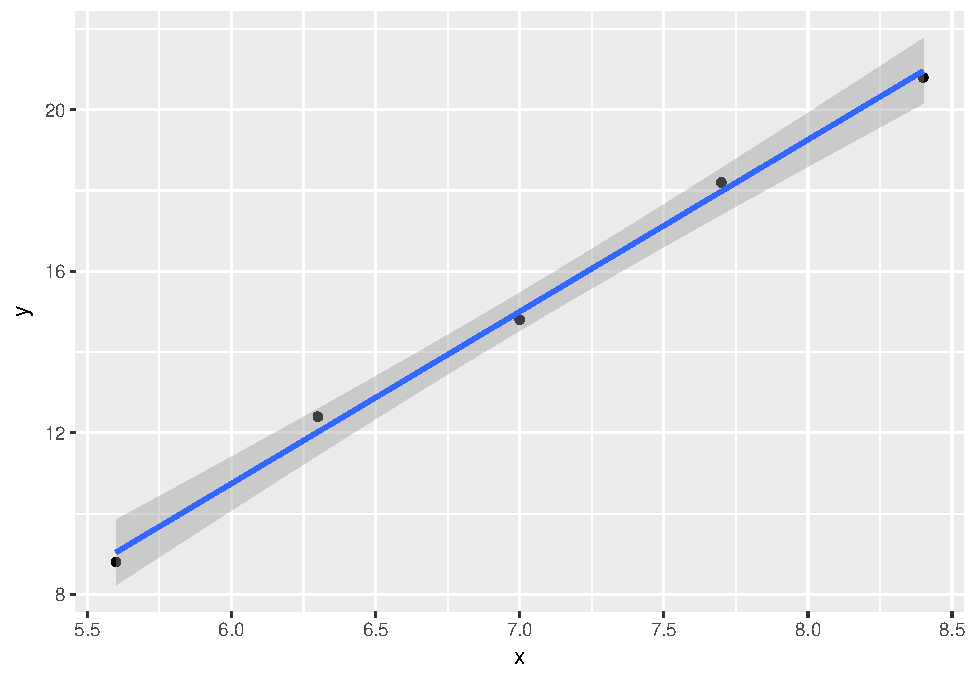
\includegraphics{DATA_605_Assignment_15_files/figure-latex/unnamed-chunk-3-1.pdf}

\hypertarget{section-1}{%
\section{2.}\label{section-1}}

Find all local maxima, local minima, and saddle points for the function
given below. Write your answer(s) in the form \((x, y, z)\). Separate
multiple points with a comma.

\[
f(x, y) = 24x - 6xy^2 - 8y^3
\]

\hypertarget{solution-1}{%
\subsection{Solution}\label{solution-1}}

We first need to find the first and second partial derivatives.

\(f_x = 24 - 6y^2\) ~ \(f_y = -12xy - 24y^2\)

\(24 - 6y^2 = 0 \ \to \ y^2 = 4 \ \to \ y = \pm 2\)

When \(y = 2\): ~\(-12xy -24y^2 = 0 \ \to \ -24x = 96 \ \to \ x = -4\).

When \(y = -2\): ~\(-12xy -24y^2 = 0 \ \to \ 24x = 96 \ \to \ x = 4\).

Plugging these values in to get our third coordinate:

\(f(-4,2) = 24(-4) - 6(-4)(2^2) - 8(2^3) =\) -64.

\(f(4,-2) = 24(4) - 6(4)(-2^2) - 8(-2^3) =\) 64.

Our two critical points are \((-4,2,-64)\) and \((4,-2,64)\).

To classify these extrema, we can use the second derivative test.

\(D(x,y) = f_{xx}f_{yy} - f_{xy}^2\).

\(f_{xx} = 0\).

\(f_{yy} = -12x - 48y\).

\(f_{xy} = f_{yx} = -12y\).

\(D = 0 - (-12y)^2 = -144y^2\).

\(D(x,y) < 0 \ \forall (x,y)\), so both critical points are saddle
points.

\hypertarget{section-2}{%
\section{3.}\label{section-2}}

A grocery store sells two brands of a product, the ``house'' brand and a
``name'' brand. The manager estimates that if she sells the ``house''
brand for \(x\) dollars and the ``name'' brand for \(y\) dollars, she
will be able to sell \(81 - 21x + 17y\) units of the ``house'' brand and
\(40 + 11x - 23y\) units of the ``name'' brand. ~ Step 1. Find the
revenue function \(R(x, y)\). ~ Step 2. What is the revenue if she sells
the ``house'' brand for \$2.30 and the ``name'' brand for \$4.10?

\hypertarget{solution-2}{%
\subsection{Solution}\label{solution-2}}

Step 1: The revenue function is simply the number of units sold
multipled by the price.

\(R(x,y) = (81 - 21x + 17y)x + (40 + 11x - 23y)y\).

Step 2: Plug in \(x = 2.30\) and \(y = 4.10\).

\(R(2.30, 4.10) = \Big[81 - 21(2.30) + 17(4.10)\Big]\times 2.30 + \Big[40 + 11(2.30) - 23(4.10)\Big]\times 4.10\)

\(R(2.30, 4.10) =\) 116.62.

\hypertarget{section-3}{%
\section{4.}\label{section-3}}

A company has a plant in Los Angeles and a plant in Denver. The firm is
committed to produce a total of 96 units of a product each week. The
total weekly cost is given by
\(C(x,y) = \frac{1}{6}x^2 + \frac{1}{6}y^2 + 7x + 25y + 700\), where
\(x\) is the number of units produced in Los Angeles and \(y\) is the
number of units produced in Denver. How many units should be produced in
each plant to minimize the total weekly cost?

\hypertarget{solution-3}{%
\subsection{Solution}\label{solution-3}}

Total units produced each week = Units produced in Los Angeles + Units
produced in Denver.

We're given \(x + y = 96\). We need to find the critical points of
\(C(x,y)\), and then find the local minimum.

Solve for either variable: \(x = y - 96, \ \ y = 96 - x\).

\begin{align*}
C(x, 96 - x) &= \frac{1}{6}x^2 + \frac{1}{6}(96 - x)^2 + 7x + 25(96 - x) + 700 \\
&= \frac{1}{6}x^2 + 1536 - 32x + \frac{1}{6}x^2 + 7x + 2400 - 25x + 700 \\
&= \frac{1}{3}x^2 - 50x + 4636 \\
C_x &= \frac{2}{3}x - 50 = 0 \\
x &= 75 \\
C_{xx} &= \frac{2}{3}
\end{align*}

Since the second derivative is \textgreater{} 0, then, by the Second
Derivative Test, there is a local minimum at 75.

Thus, the Los Angeles plant should produce 75 units, and the Denver
plant should produce 21 units.

\hypertarget{section-4}{%
\section{5.}\label{section-4}}

Evaluate the double integral on the given region. Write your answer in
exact form without decimals.

\[
\iint \limits_R (e^{8x + 3y})dA; \ \ R: 2 \leq x \leq 4 \ \ \text{and } \ 2 \leq y \leq 4
\]

\hypertarget{solution-4}{%
\subsection{Solution}\label{solution-4}}

\begin{align*}
&\int\limits_{2}^{4} \int\limits_{2}^{4} (e^{8x + 3y}) \ dx \ dy \\
&\int\limits_{2}^{4} e^{8x} \ dx \int\limits_{2}^{4} e^{3y} \ dy \\
&\frac{1}{8}e^{8x}\Big|_{2}^{4} \cdot \frac{1}{3}e^{3y}\Big|_{2}^{4} \\
&\frac{1}{24}(e^{32} - e^{16})(e^{12} - e^{6})
\end{align*}

\begin{Shaded}
\begin{Highlighting}[]
\NormalTok{(}\DecValTok{1}\OperatorTok{/}\DecValTok{24}\NormalTok{)}\OperatorTok{*}\NormalTok{((}\KeywordTok{exp}\NormalTok{(}\DecValTok{32}\NormalTok{) }\OperatorTok{-}\StringTok{ }\KeywordTok{exp}\NormalTok{(}\DecValTok{16}\NormalTok{))}\OperatorTok{*}\NormalTok{(}\KeywordTok{exp}\NormalTok{(}\DecValTok{12}\NormalTok{) }\OperatorTok{-}\StringTok{ }\KeywordTok{exp}\NormalTok{(}\DecValTok{6}\NormalTok{)))}
\NormalTok{## [1] 5.341559e+17}
\end{Highlighting}
\end{Shaded}


\end{document}
